% Compléments
\subsection{Compléments}

% Descente de gradient
\begin{frame}
    \frametitle{Un cas de non convergence de la descente de gradient}
    \begin{figure}
        \centering
        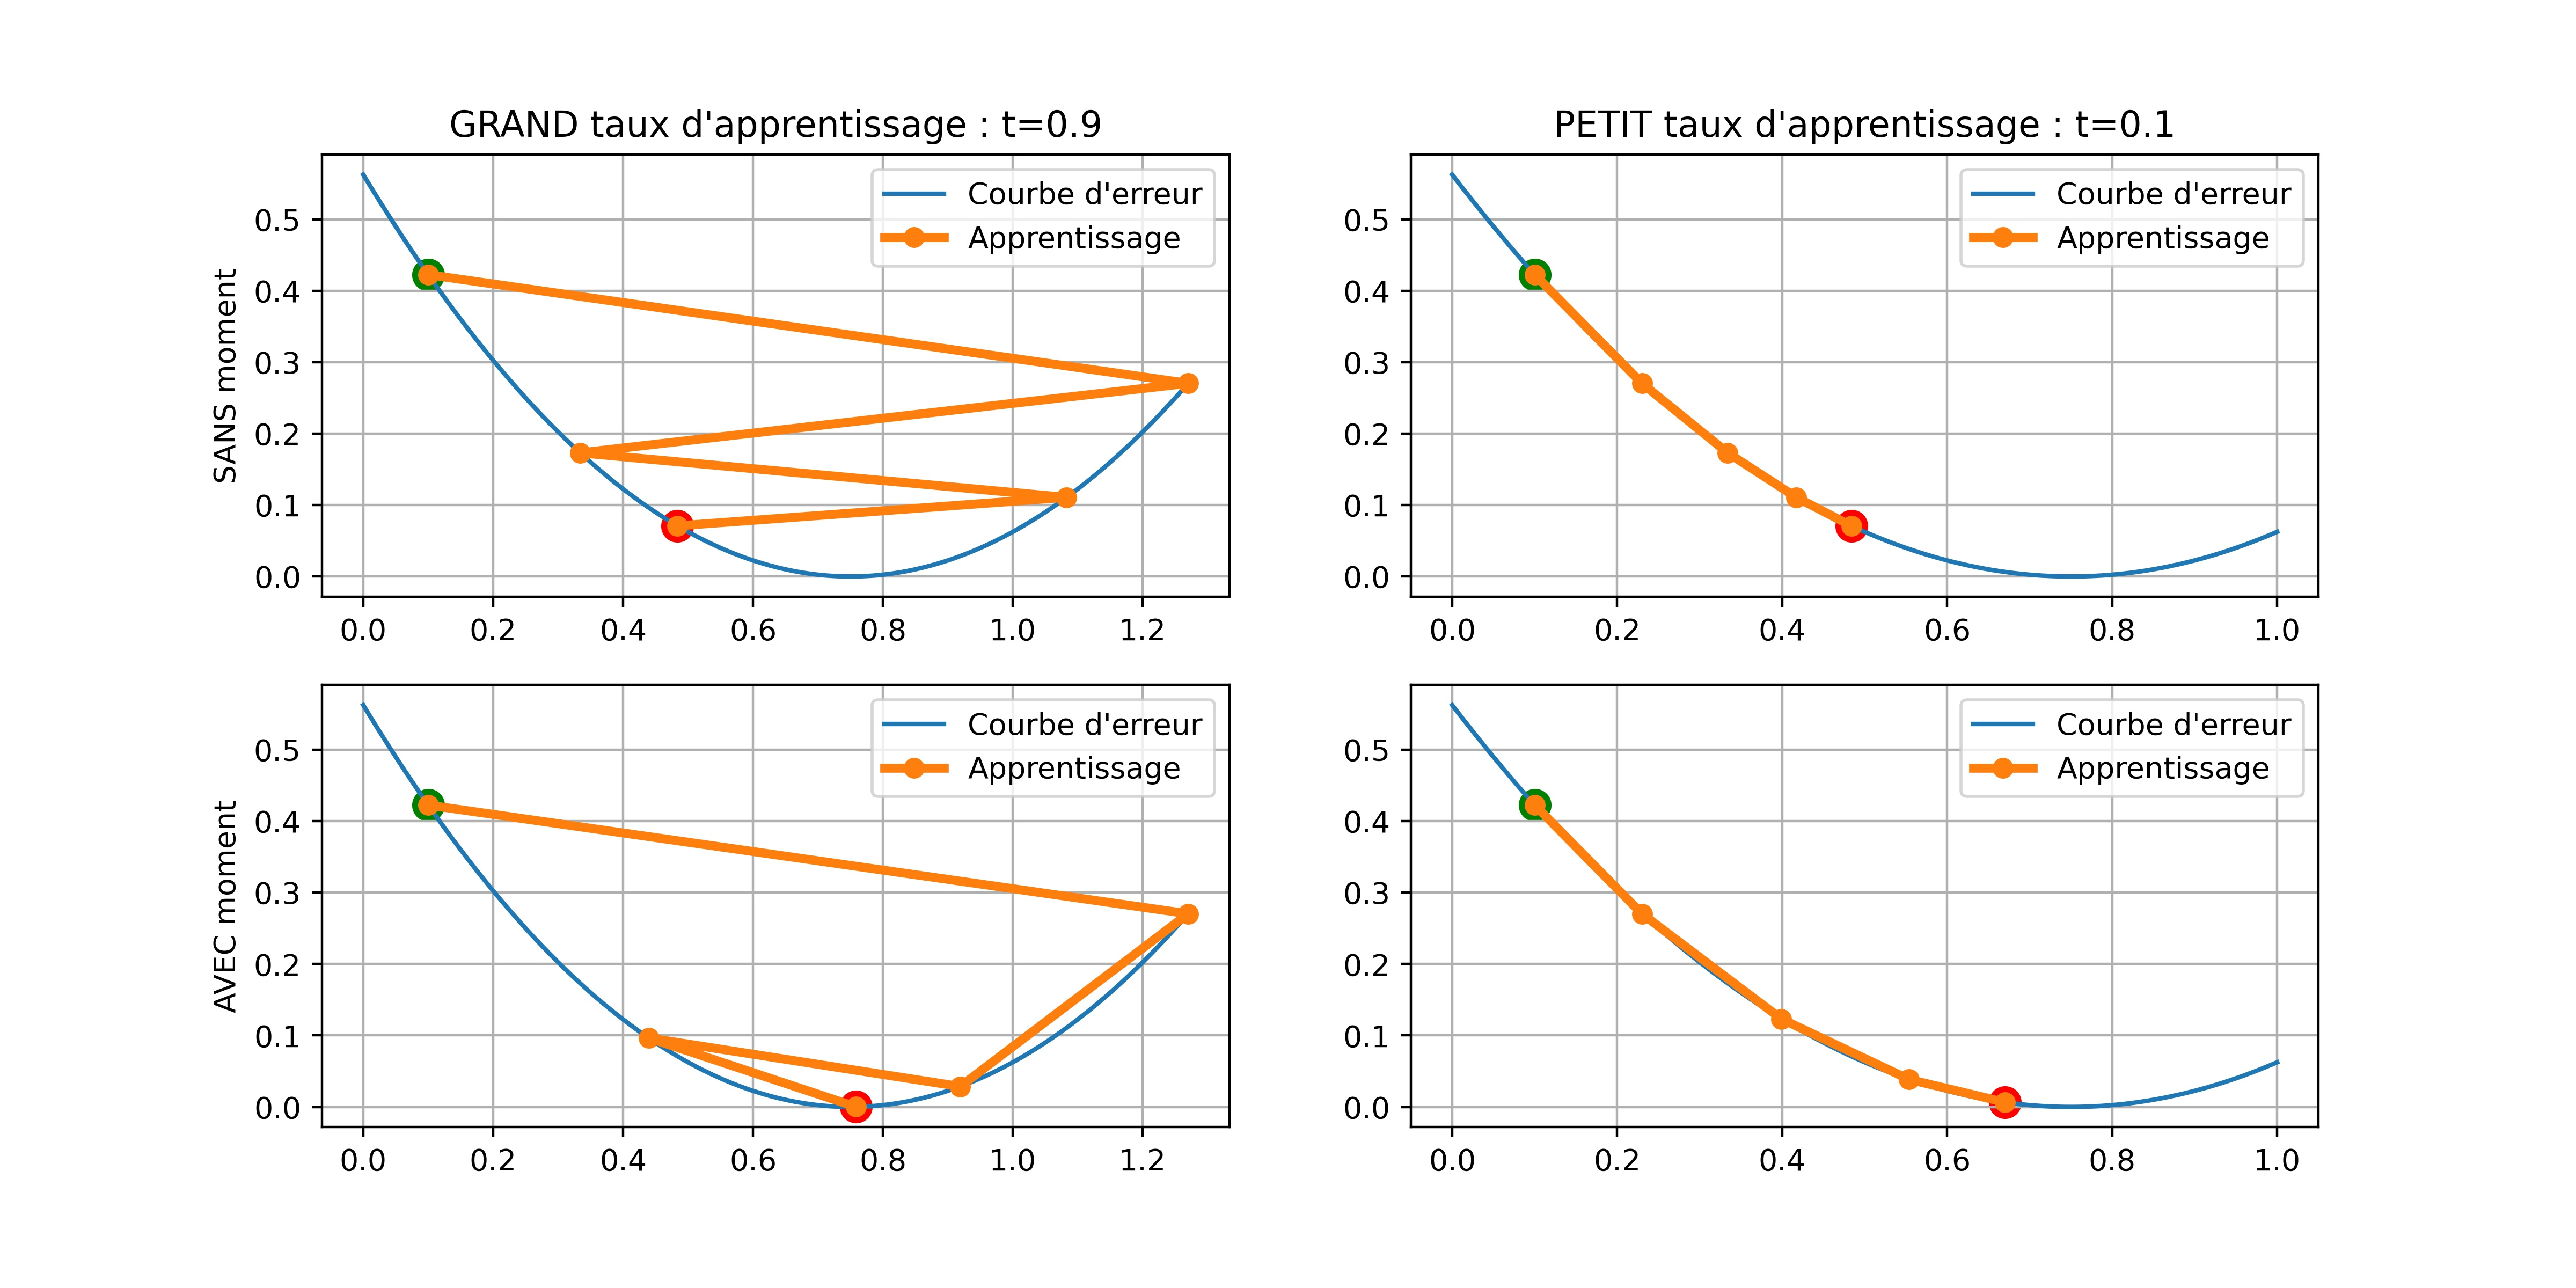
\includegraphics[height=120px]{3-Moment.jpg}
        \caption{Descente de gradient SANS/AVEC momentum où $\gamma = 0.5$}
    \end{figure}
\end{frame}

\begin{frame}{La terminaison de la descente de gradient}
    \begin{block}{En pratique}
        Pour terminer les itérations de la rétropropagation sur un réseau de neurones trois conditions de terminaison existent :
        \begin{itemize}
            \item Un nombre maximal d'itération de la rétropropagation
            \item Un seuil minimal pour l'erreur
            \item Un seuil minimal pour la norme infinie du gradient
        \end{itemize}
        Ainsi, en pratique, si une de ces trois conditions est atteinte, l'algorithme se termine. Le variant de boucle du nombre d'itérations assure alors la terminaison de l'algorithme
    \end{block}
\end{frame}

\begin{frame}{Les hypothèses pour la terminaison}
    \begin{alertblock}{En théorie}
        Une fonction de $R^n$ dans $R$ de classe $C^2$, strictement convexe et coercive ($\lim_{\lVert x \rVert \to+\infty} f(x) = +\infty$) admet un unique minimum. On peut donc trouver une suite $t_k$ de taux d'apprentissage de sorte que la descente de gradient converge.
    \end{alertblock}
    \begin{exampleblock}{Exemple avec les hypothèses}
        La relation de récurrence s'écrit alors : \\
        \begin{center}
            \centering
                $x_{k+1} = x_k - t_k \nabla f(x_k)$
        \end{center}
        avec $x_k$ tendant vers l'unique minimum de $f$
    \end{exampleblock}
\end{frame}

\begin{frame}{La rétropropagation sur le XOR}
    \begin{figure}
        \centering
        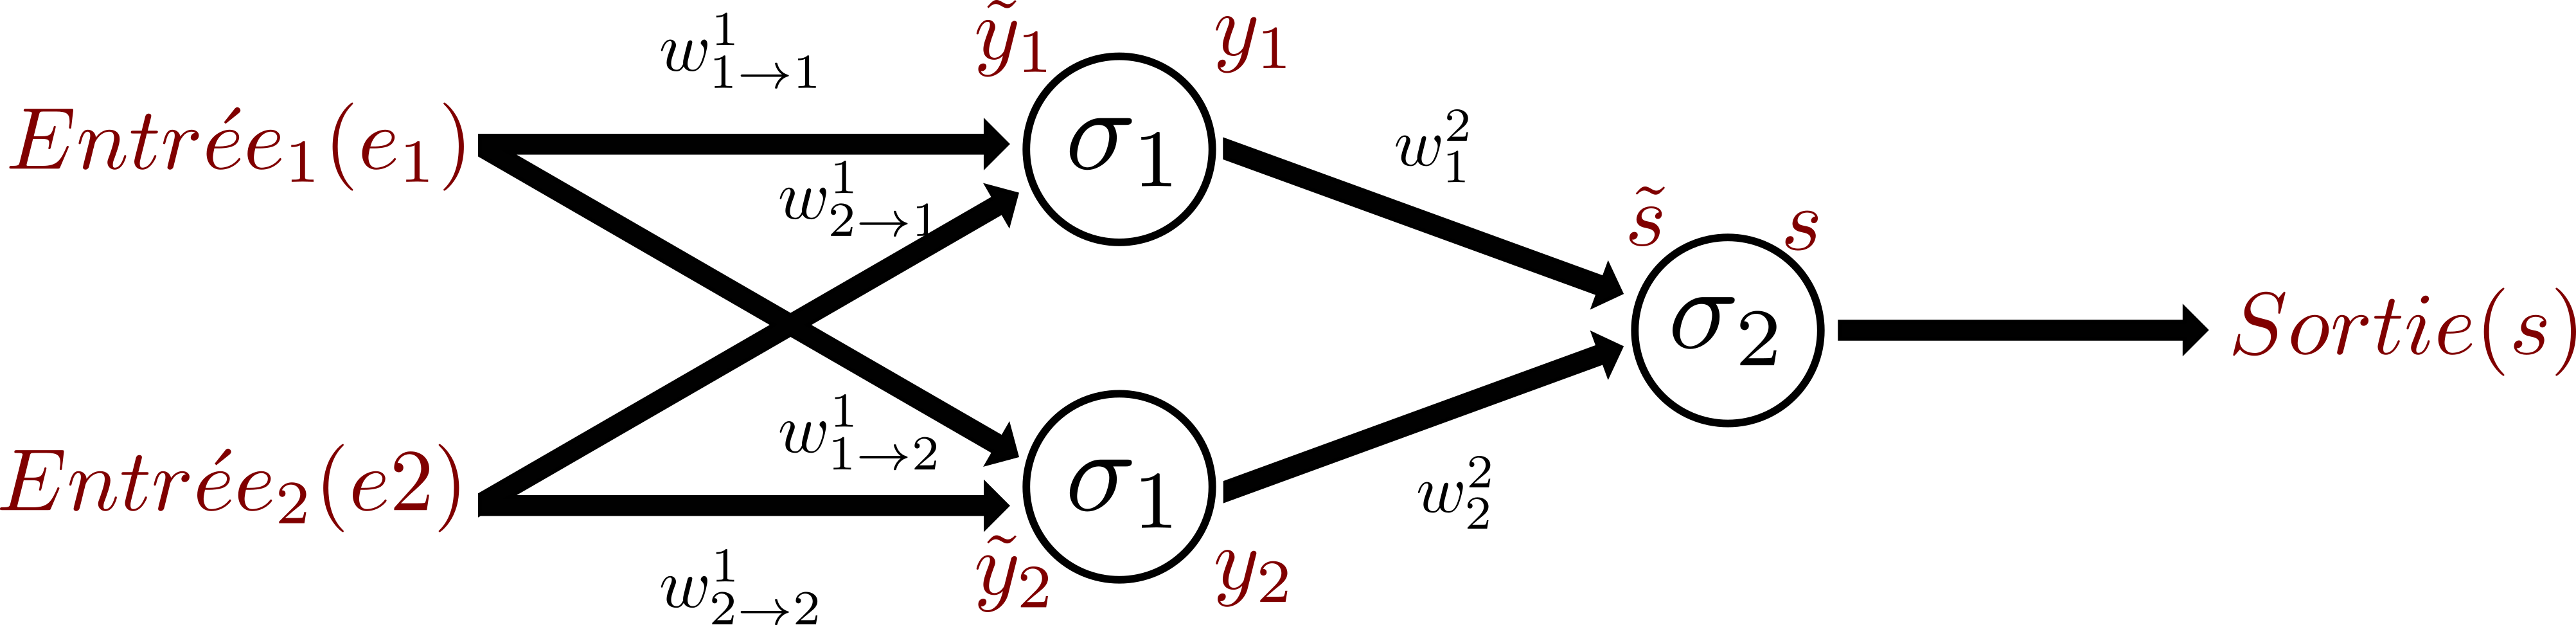
\includegraphics[width=\textwidth]{5-Model.png}
        \caption{Schéma du réseau de neurones reproduisant le XOR}
    \end{figure}
    \begin{equation}
        \begin{cases}
            \tilde{y}_1 = w^1_{11}\times e_1 +  w^1_{21}\times e_2 \\
            \tilde{y}_2 = w^1_{12}\times e_1 +  w^1_{22}\times e_2 \\
            \tilde{s}   = w^2_{1}\times y_1 +  w^1_{11}\times y_2  \\
        \end{cases}
        et
        \begin{cases}
            y_1 = \sigma_1(\tilde{y}_1) \\
            y_2 = \sigma_1(\tilde{y}_2) \\
            s = \sigma_2(\tilde{s})     \\
        \end{cases}
    \end{equation}
\end{frame}

\begin{frame}{Une simplification matricielle}
    \begin{block}{Convention adoptée}
        \begin{description}
            \item[@] Le produit matriciel
            \item[*] Le produit d'Hadamard
            \item[$f$] La fonction d'erreur $f:s \rightarrow (s-s_{attendue})^2$
        \end{description}
    \end{block}
    \begin{equation}
        \begin{cases}
            \begin{pmatrix}
                \tilde{y}_1 \\
                \tilde{y}_2
            \end{pmatrix}
            =
            \begin{pmatrix}
                w^1_{11} & w^1_{21} \\
                w^1_{12} & w^1_{22}
            \end{pmatrix}
            @
            \begin{pmatrix}
                e_1 \\
                e_2
            \end{pmatrix}\\
            \begin{pmatrix}
                \tilde{s}
            \end{pmatrix}
            =
            \begin{pmatrix}
                w^2_{1} & w^2_{2}
            \end{pmatrix}
            @
            \begin{pmatrix}
                y_1 \\
                y_2
            \end{pmatrix}
        \end{cases}
    \end{equation}
\end{frame}

\begin{frame}{La rétropropagation matricielle}
    \begin{equation}
        \begin{cases}
            \begin{pmatrix}
                \frac{\partial f}{\partial w^2_1}(w^2_1)  & \frac{\partial f}{\partial w^2_2}(w^2_1) \\
               
            \end{pmatrix}
            =
            \begin{pmatrix}
                \frac{\partial f}{\partial s}(s)
            \end{pmatrix}
            *
            \begin{pmatrix}
                \sigma_2 '(\tilde{s}) 
            \end{pmatrix}
            @ 
            \begin{pmatrix}
                y_1 \\
                y_2
            \end{pmatrix} ^t

            \\
            \begin{pmatrix}
                \frac{\partial f}{\partial w^2_{11}}(w^2_{11})  & \frac{\partial f}{\partial w^2_{21}}(w^2_{21}) \\
                \frac{\partial f}{\partial w^2_{12}}(w^2_{12}) & \frac{\partial f}{\partial w^2_{22}}(w^2_{22})
            \end{pmatrix}
            =
            \begin{pmatrix}
                \frac{\partial f}{\partial y_1}(y_1) \\
                \frac{\partial f}{\partial y_2}(y_2)
            \end{pmatrix}
            *
            \begin{pmatrix}
                \sigma_1 '(\tilde{y}_1) \\
                \sigma_1 '(\tilde{y}_2)
            \end{pmatrix}
            @ 
            \begin{pmatrix}
                e_1 \\
                e_2
            \end{pmatrix} ^t
        \end{cases}
    \end{equation}
    avec
    \begin{equation}
        \begin{cases}
            \begin{pmatrix}
                \frac{\partial f}{\partial y_1}(y_1) \\
                \frac{\partial f}{\partial y_2}(y_2)
            \end{pmatrix} ^t
            =
            \begin{pmatrix}
                \frac{\partial f}{\partial s}(s) 
            \end{pmatrix}
            *
            \begin{pmatrix}
                \sigma_2 '(\tilde{s}) 
            \end{pmatrix}
            @
            \begin{pmatrix}
                w^2_1 & w^2_2                
            \end{pmatrix}
        \end{cases}
    \end{equation}
\end{frame}

% Fonction d'activation
\begin{frame}{Des fonctions d'activation}
    \begin{block}{}
        \centering
        \begin{tabular}{ l || c | c | }
            Fonction                        & Formule                                          & Dérivée                                     \\ \hline \\
            Sigmoïde                        & $\mathlarger{\frac{1}{1+e^{-x}}}$                & $f(x) \times (1-f(x))$                      \\ \\
            Tangente Hyperbolique (Tanh)    & $\mathlarger{\frac{e^{x}-e^{-x}}{e^{x}+e^{-x}}}$ & $1-f(x)^2$                                  \\ \\
            Unité Linéaire Rectifiée (ReLU) & $max(0, x)$                                      & $ \left\{\begin{array}{ll}
                    0 & \mbox{si } x<0 \\
                    1 & \mbox{sinon }\end{array}\right.$ \\
        \end{tabular}
    \end{block}
\end{frame}

\begin{frame}{La fonction d'activation : Sigmoïde}
    \begin{figure}
        \centering
        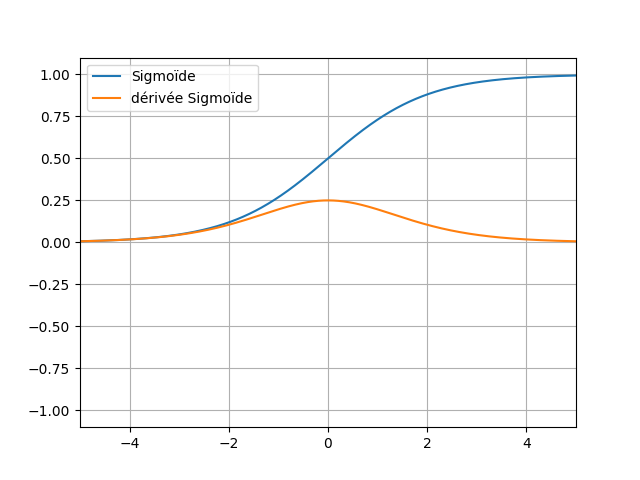
\includegraphics[width=220px]{0-Sigmoide.png}
        \caption{Sigmoïde}
    \end{figure}
\end{frame}

\begin{frame}{La fonction d'activation : TANH}
    \begin{figure}
        \centering
        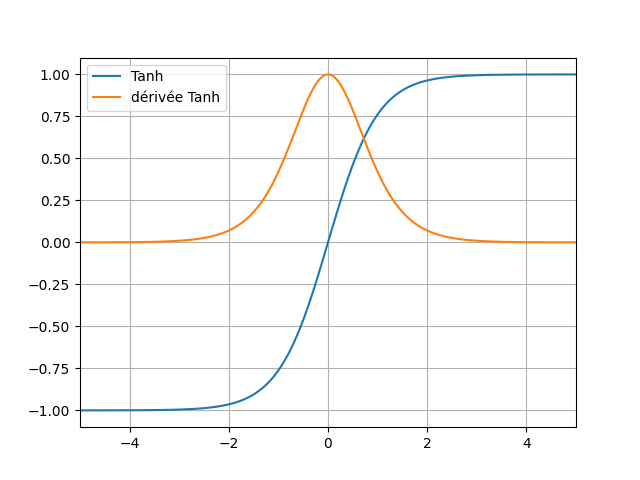
\includegraphics[width=220px]{0-Tanh.png}
        \caption{TANH}
    \end{figure}
\end{frame}

\begin{frame}{La fonction d'activation : ReLu}
    \begin{figure}
        \centering
        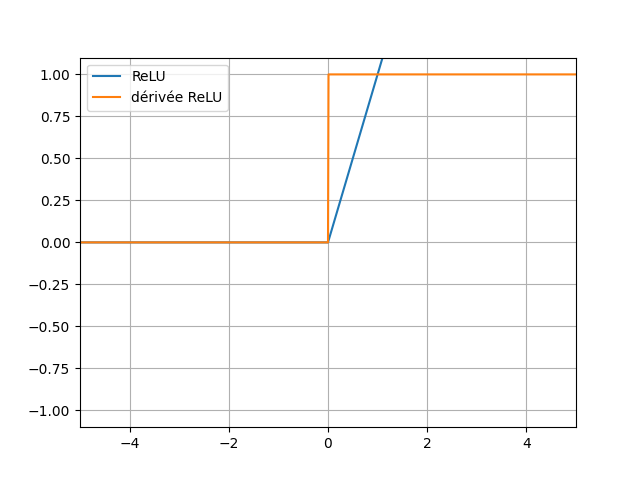
\includegraphics[width=220px]{0-ReLU.png}
        \caption{ReLu}
    \end{figure}
\end{frame}

% La rétropropagation classification
\begin{frame}{La rétropropagation pour la classification}
    \begin{block}{Cross-entropy}
        La fonction d'erreur des problèmes de classification est Cross-entropy : \\
        • $L\ \ \ = -\sum_{k=1}^{n}y_ilog(p_i)$ avec $y_i$ la sortie attendue \\
        • $\dfrac{\partial L}{\partial a_i} = p_i - y_i$
    \end{block}
\end{frame}


% Reconnaissance d'image de vêtement

\begin{frame}{Une base de données plus complexe}
    \begin{block}{Description}
        Images de taille $28 \times 28$ pixels en noir et blanc : \\
        \quad - 60 000 images pour l'entrainement. \\
        \quad - 10 000 autres pour la vérification.
    \end{block}
    \begin{columns}
        \begin{column}{0.5\textwidth}
            \begin{figure}
                \centering
                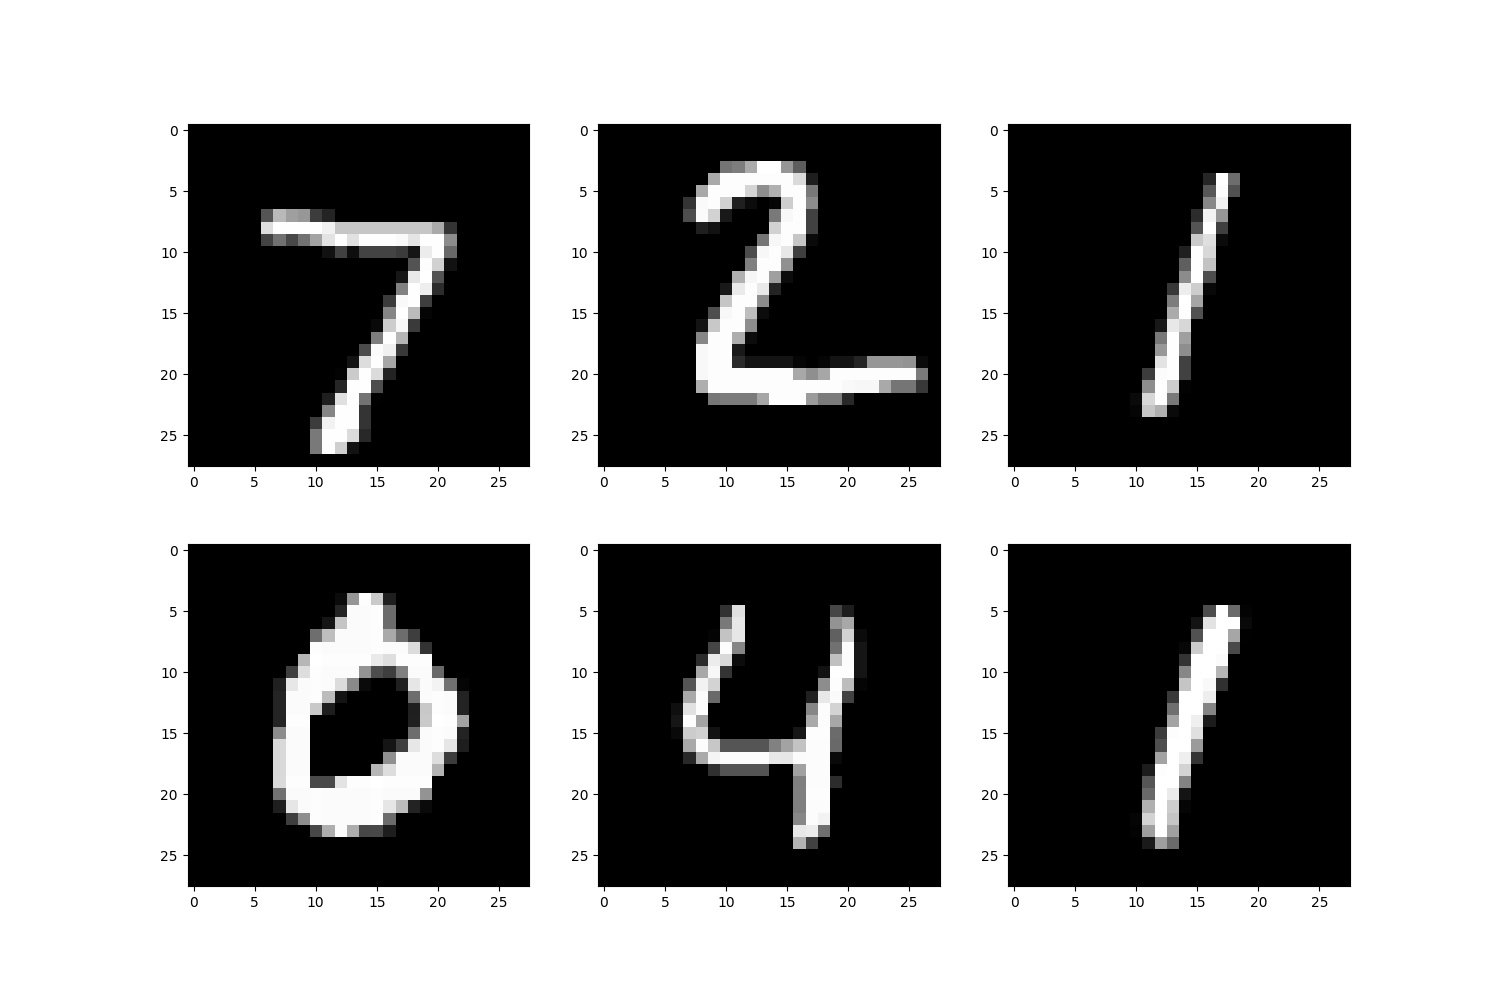
\includegraphics[width=\textwidth]{1-mnist.jpg}
                \caption{MNIST}
            \end{figure}
        \end{column}
        \begin{column}{0.5\textwidth}
            \begin{figure}
                \centering
                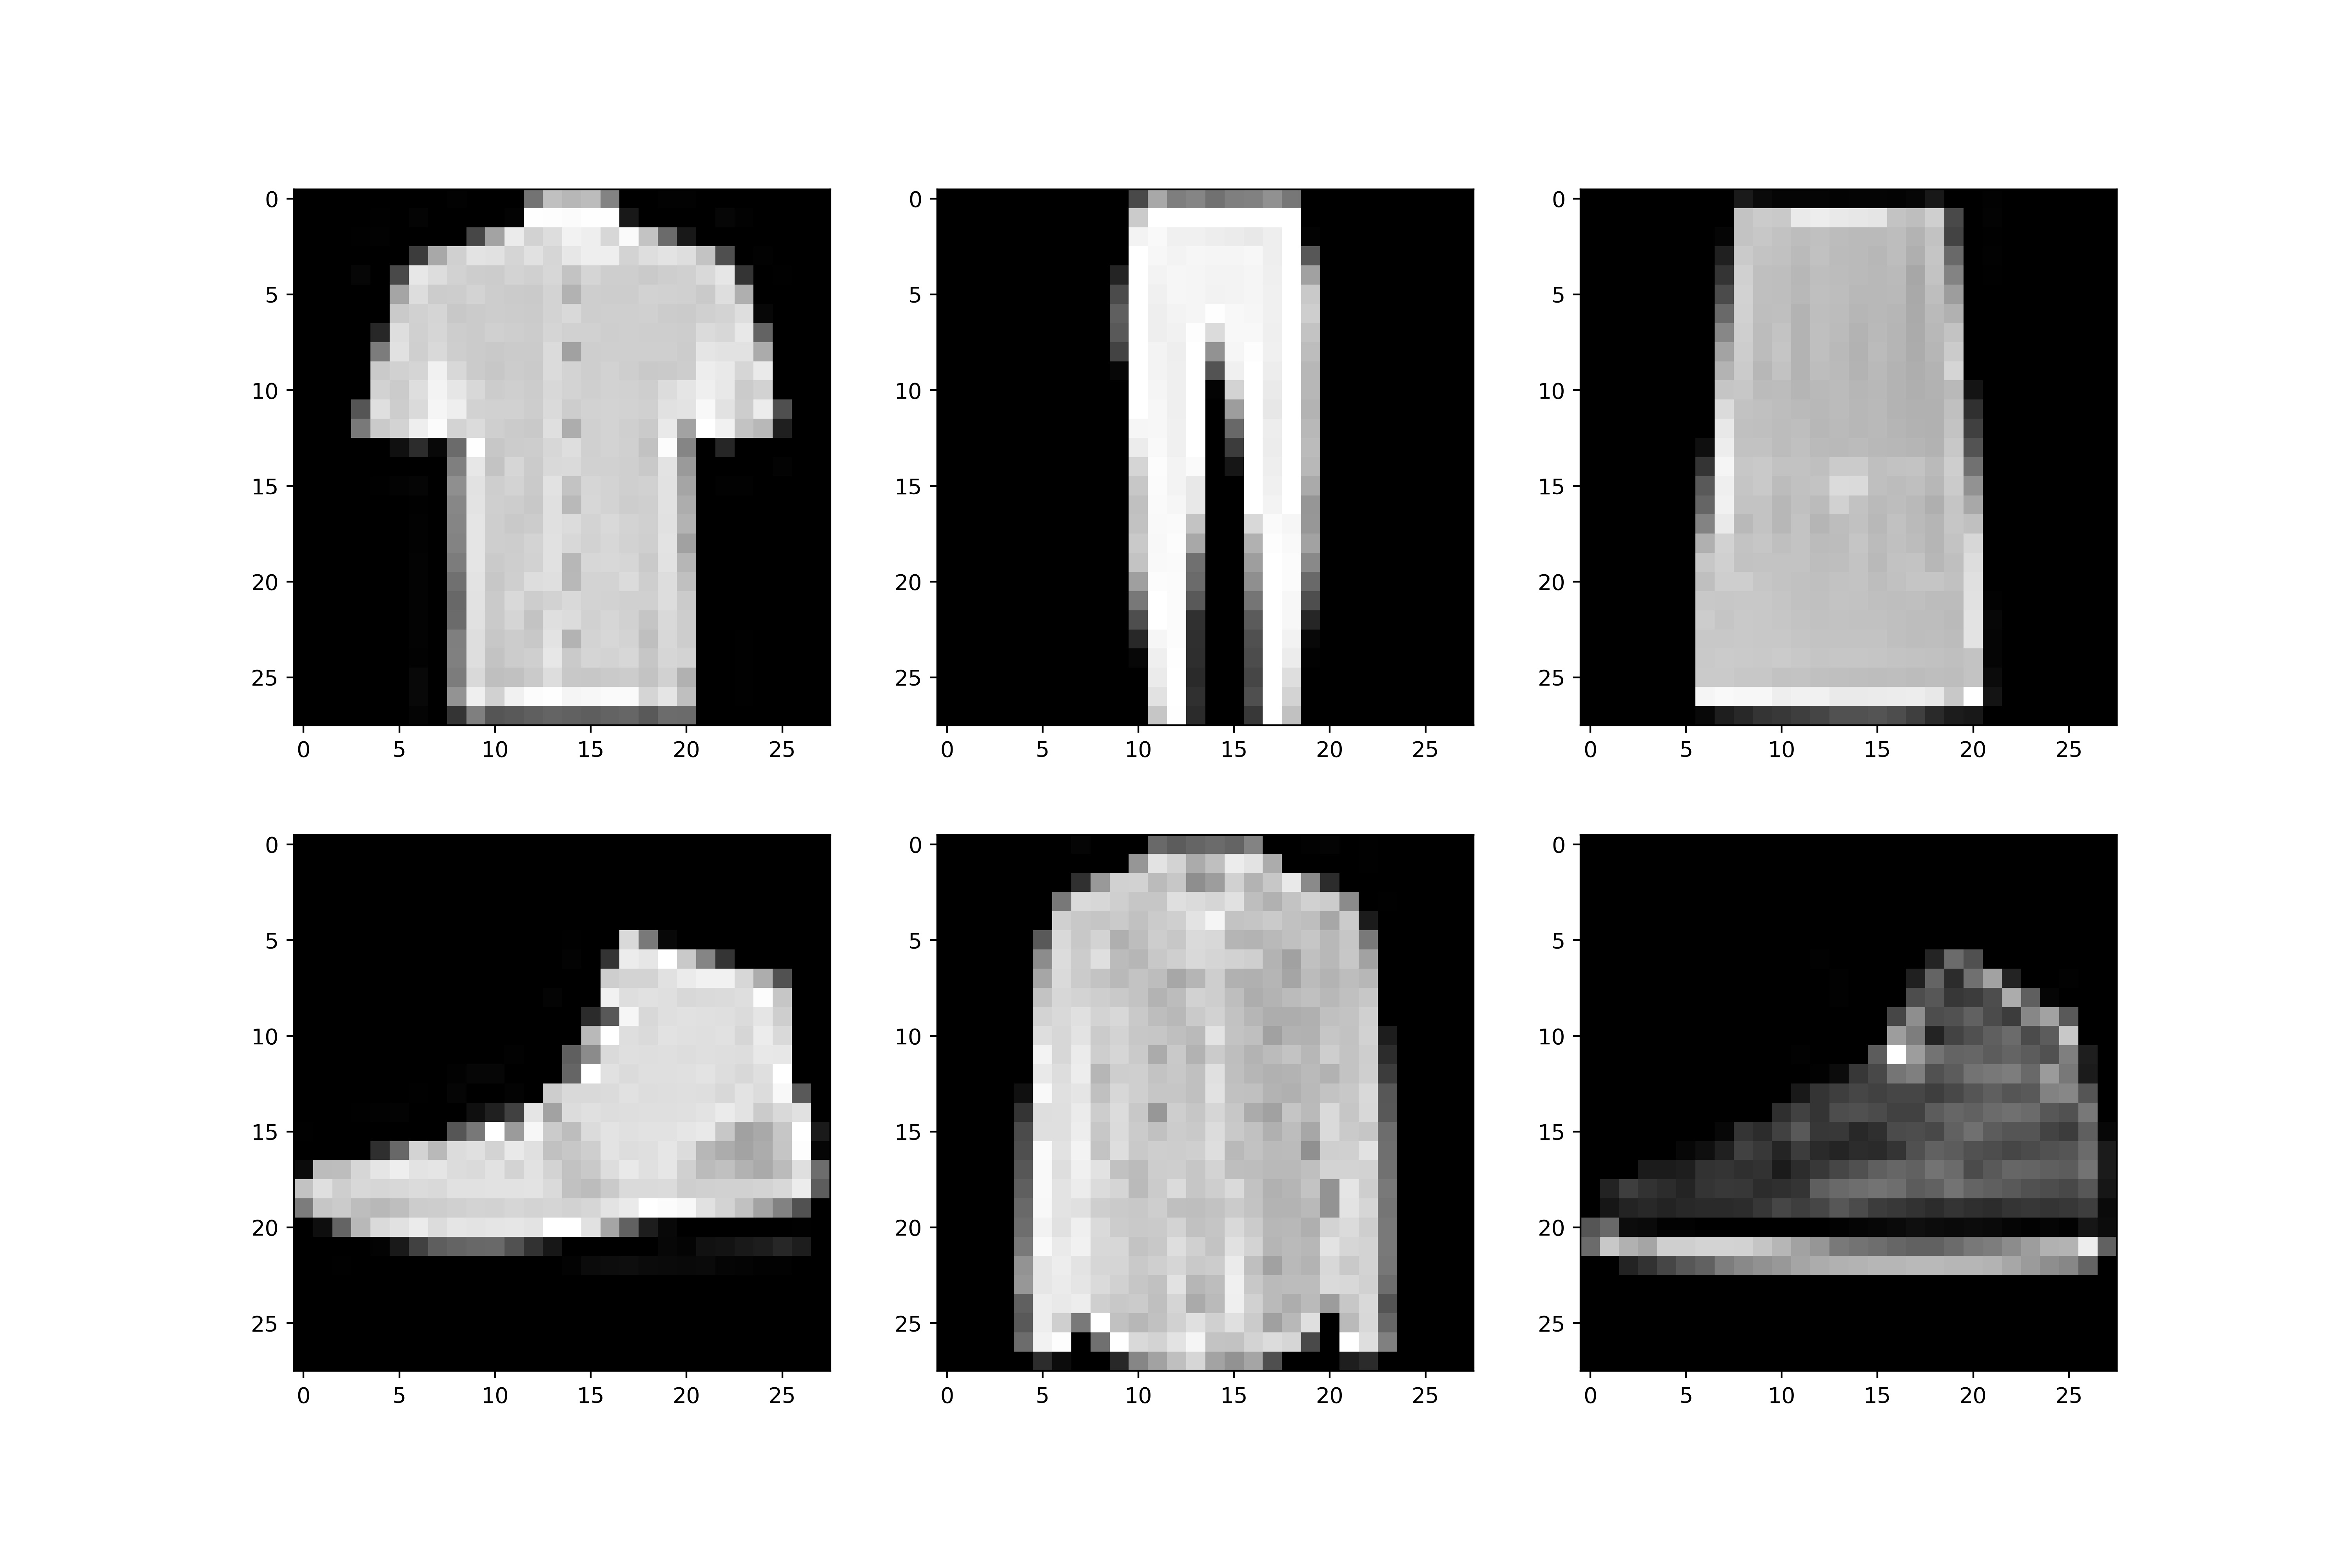
\includegraphics[width=\textwidth]{8-fashion-mnist.jpg}
                \caption{Fashion MNIST}
            \end{figure}
        \end{column}
    \end{columns}
\end{frame}


\begin{frame}{Mes résultats}
    \begin{columns}[T]
        \begin{column}{.75\textwidth}
            \begin{figure}
                \centering
                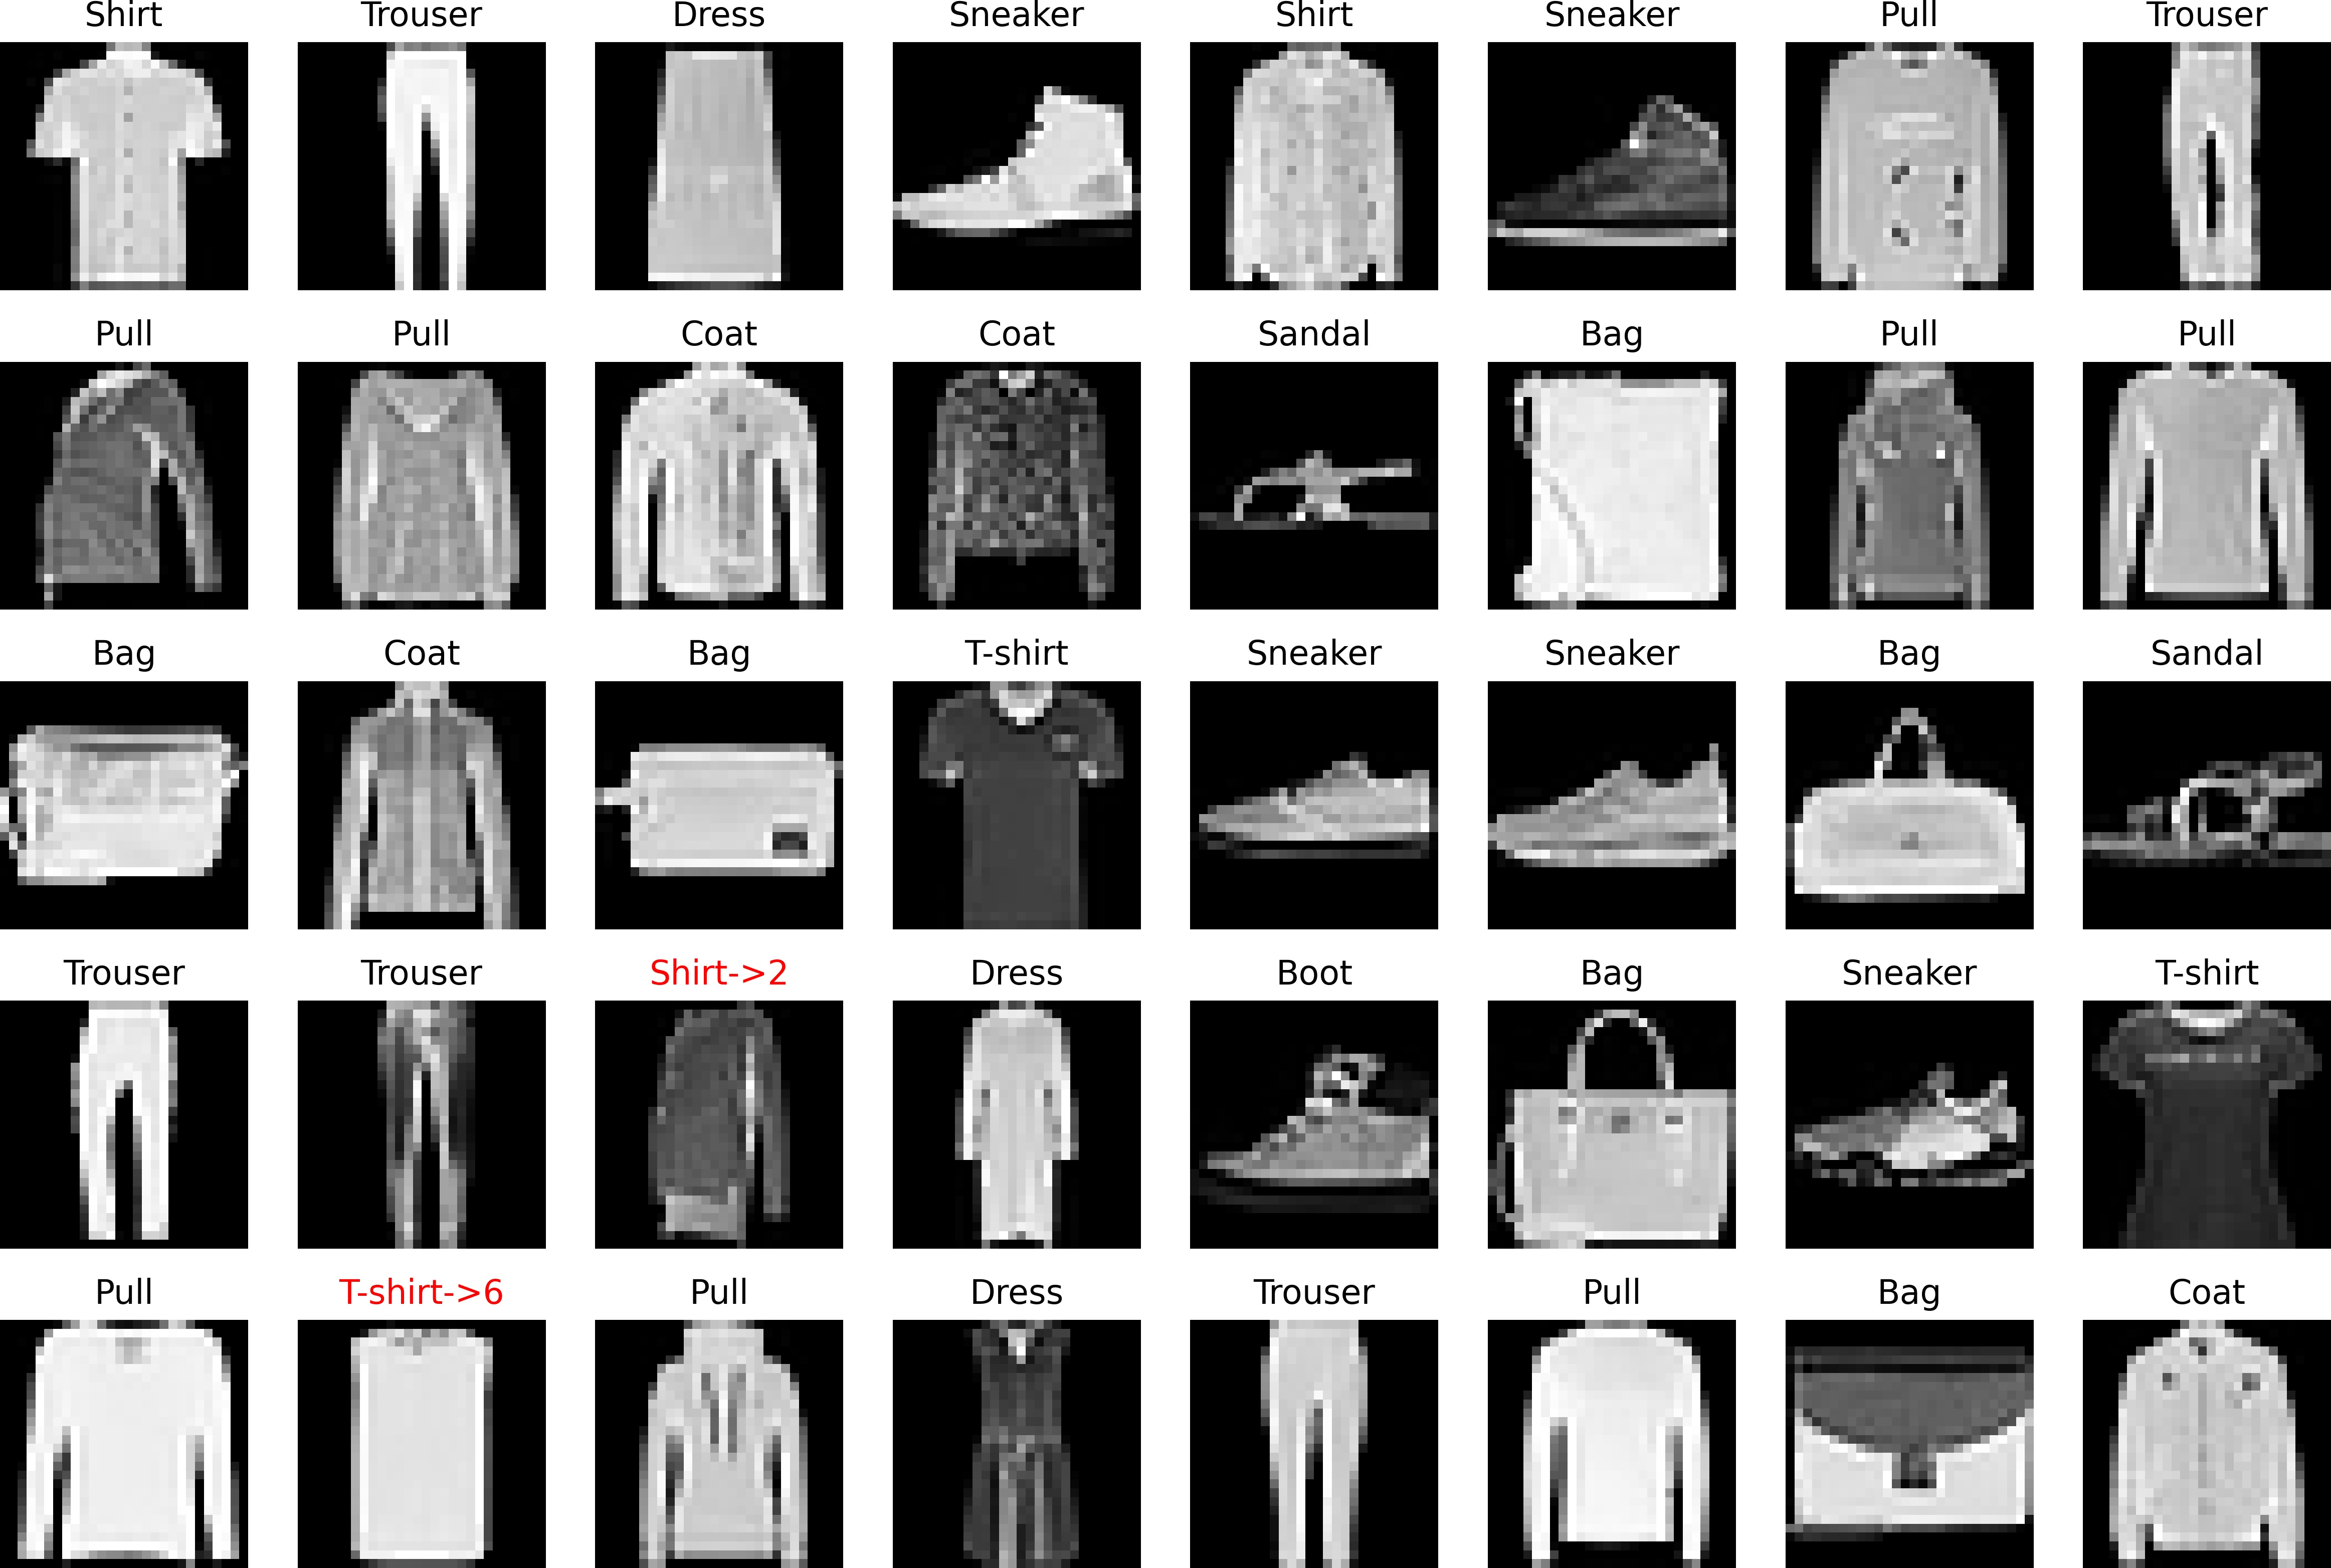
\includegraphics[width=\textwidth]{7-Resultat.jpg}
                \caption{Exemple sur un échantillon de 40 images $Fashion\ MNIST$}
            \end{figure}
        \end{column}
        \hfill
        \begin{column}{.25\textwidth}
            \bigskip	\bigskip	\bigskip
            \lstinputlisting[language=Python, firstline=15]{6-fashionDico.py}
        \end{column}
    \end{columns}
\end{frame}



% Transfert d'apprentissage
\begin{frame}[fragile]{Réseau de neurones modèle}
    \lstinputlisting[language=Python]{7-model}
\end{frame}

\begin{frame}[fragile]{Réseau de neurones adapté}
    \lstinputlisting[language=Python]{9-model2}
\end{frame}